% !TeX program = pdflatex
% !TeX encoding = UTF-8
\documentclass[fontsize=11pt, parskip=half]{scrartcl}

%preamble loading packages and so on

%packages
\usepackage{scrlayer-scrpage}
\usepackage[datesep={.}, style=ddmmyyyy]{datetime2}
\usepackage{graphicx}
\usepackage{multicol}
\usepackage[colorlinks=true, urlcolor=blue, linkcolor=black]{hyperref}
\usepackage{amsmath}
\usepackage{mathtools}
\usepackage{listings}
\usepackage{csquotes}
\usepackage{wrapfig}
\usepackage{caption}
\usepackage[a4paper, top=2cm, bottom=2cm, left=2cm, right=2cm]{geometry}
\MakeOuterQuote{"}
\usepackage{array}   % for \newcolumntype macro
\usepackage{multirow}
\newcolumntype{L}{>{$}l<{$}} % math-mode version of "l" column type
\newcolumntype{C}{>{$}c<{$}} % math-mode version of "c" column type
\newcolumntype{R}{>{$}r<{$}} % math-mode version of "r" column type

%%%%%%%%%%%%%%
%commands
%%%%%%%%%%%%%%

%formatting
\renewcommand{\thesubsection}{\thesection.H\arabic{subsection}} %changes subsection labelling to alphabetical -> 1.a instead of 1.1
\captionsetup{labelfont=bf, textfont=it, justification=raggedright,singlelinecheck=false, justification=centering}
%generalmath
\newcommand\br[1]{\ensuremath{\left(#1\right)}}
\newcommand\modulo[1]{\ensuremath{\bmod{\left(#1\right)}}} %adds \modulo{} as command for modulo calculations. Content is placed in brackets.
\DeclarePairedDelimiter\ceil{\lceil}{\rceil} %defines \ceil{} as command producing mathematical ceiling symbols around content
\DeclarePairedDelimiter\floor{\lfloor}{\rfloor} %defines \floor{} as command producing mathematical floor symbols around content
\newcommand\bsum[3]{\ensuremath{\sum_{#1}^{#2}{\left({#3}\right)}}} %defines \bsum{}{}{} as command for large sum with start, end and content. Content is placed in brackets.
\newcommand\bprod[3]{\ensuremath{\prod_{#1}^{#2}{\left({#3}\right)}}} %defines \bprod{}{}{} as command for large product with start, end and content. Content is placed in brackets.
\newcommand\texeq[1]{\stackrel{\mathclap{\normalfont\mbox{\scriptsize {#1}}}}{=}} %defines \teq as command for equal sign with subscript
\newcommand\defeq{\ensuremath{=_{def}}} %defines \defeq as command for definition with equal sign

%formal logic
\newcommand\bland[3]{\ensuremath{\bigwedge_{#1}^{#2}{\left({#3}\right)}}} %defines \bland{}{}{} as command for large logical AND with start, end and content. Content is placed in brackets.
\newcommand\blor[3]{\ensuremath{\bigvee_{#1}^{#2}{\left({#3}\right)}}} %defines \bland{}{}{} as command for large logical OR with start, end and content. Content is placed in brackets.
\newcommand\bforall[2]{\ensuremath{\left(\forall {#1}\right) \left[{#2}\right]}} %defines \bforall{}{} as command for logical forall with variable and content. forall and variable are placed within (), Content is placed in [].
\newcommand\bexists[2]{\ensuremath{\left(\exists {#1}\right) \left[{#2}\right]}} %defines \bexists{}{} as command for logical exists with variable and content. forall and variable are placed within (), Content is placed in [].

%Mathmatical Sets (Mengenlehre)
\newcommand\intenset[2]{\ensuremath{\left\lbrace {#1} \mid {#2} \right\rbrace}} %defines \intenset{}{} as command for intensional notation of mathmatical sets: {@|@}.
\newcommand\intensetU[2]{\ensuremath{\left\lbrace {#1} \in U \mid {#2} \right\rbrace}} %defines \intensetU{}{} as command for intensional notation of mathmatical sets: {@ \in U |@}.
\newcommand\extenset[1]{\ensuremath{\left\lbrace {#1} \right\rbrace}} %defines \extenset{} as command for extensional notation of mathmatical sets: {@}.

% referencing
\newcommand\fref[1]{\textbf{Figure \ref{#1}}} % defines \fref{} as command printing "Figure figurenumber" in bold.

%Title, Author, ...
\makeatletter
\title{Conspiracy narratives and public perception of 15-minute cities on YouTube}\let\Title\@title
\def \papersubtitle {Project Report}
\def \paperdeadline {21.08.2024}
% seminar information
\def \paperevaluator {Max Pellert}
\def \paperseminar {Social Media Data Analysis}
\def \papersemester {Summer/Winter Semester 2024}
\def \paperdepartment {Department of Politics and Public Administration}
\def \paperuniversity {University of Konstanz}
% personal information
\def \paperemail {julia.king@uni-konstanz.de}
\def \paperprogramme {M.Sc. Social and Economic Data Science}
\def \papermatriculationnr {01/911139}
\author{Julia King}          \let\Author\@author
\date{\today}           \let\Date\@date
\makeatother

% Page Layout
\ihead{Julia K.}
\chead{Conspiracy narratives \& public perception of 15-minute cities on YouTube}
\ohead{SMDA}

% caption setup
\captionsetup{labelfont=bf, textfont=it, justification=raggedright,singlelinecheck=false}

% citation setup
\usepackage[style=apa, sorting=nyt, backend=biber]{biblatex}
\usepackage{etoolbox} % If not already included
\addbibresource{citations.bib} %bibliography file


% Custom bibliography driver for article to include howpublished
\DeclareBibliographyDriver{misc}{%
  \printnames{author}%
  \newunit\newblock
  \printfield{year}%
  \newunit\newblock
  \mkbibemph{\printfield{title}}.%
  \newunit\newblock
  \iffieldundef{howpublished}
    {}
    { \href{\thefield{howpublished}}{\thefield{howpublished}}}%
  \newunit\newblock
  \printfield{url}%
}

\begin{document}
\setlength{\columnsep}{25pt}

% Title Page, do not change here, variables are defined above!
\begin{titlepage}
    \newcommand{\HRule}{\rule{\linewidth}{0.5mm}}
    
    \begin{flushleft} % Upper left corner
        \large
        \paperuniversity\\
        \paperdepartment\\
        \papersemester\\
        \paperseminar\\
        \paperevaluator
    \end{flushleft}
    
    \vfill
    
    \begin{center} % Centered title and date
        \huge\bfseries \Title\\
        \vspace{0.5cm}
        \large \papersubtitle \\
        \vspace{0.5cm}
        \small Deadline: \paperdeadline
    \end{center}
    
    \vfill
    
    \begin{flushright} % Lower right corner
        \large
        \Author\\
        \papermatriculationnr\\
        \paperprogramme\\
        \paperemail
    \end{flushright}
\end{titlepage}

\clearpage
\setcounter{page}{1}

% Main Document
\section{Motivation}
\label{section:motivation}

    The concept of a 15-minute-city is, in and of itself, nothing more than an architectural proposal for efficient and sustainable urban design. However, it rose to prominence during the past five years due to a staggering amount of online conspiracy theories and misinformation. While conspiracy theories often revolve around large events or hard-to-explain phenomena, like the moon landing or many celebrity or politician assassinations, 15-minute-cities are neither. 15-minute-cities, in contrast, are a suggestion in the research field of architecture and city planning, proposing to build new urban developments in a way that ensures residents can reach basic amenities within a 15-minute walking distance. The fact that a simple, academic proposal for city design was (and is) the center of large swathes of online conspiracy theories, is puzzling, and warrants investigation. 
    
    Understanding the puzzling emergence of 15-minute-city conspiracies requires investigation of the ways in which people discussed them publicly. This project aims, therefore, to track the development of theories revolving around this concept by analyzing the online discourse around it. This requires an in-depth understanding of the process in which conspiracy theories took over the discourse on 15-minute-cities. Consequently, this project collects metrics on the viewership of online videos revolving around 15-minute-cities, and to classify the discursive tone of both the videos themselves and the comments posted on them. Using this data, the following hypotheses are tested: 

    \begin{enumerate}
        \item Videos produced before the first spike in public interest are more likely to be non-conspirative compared to those uploaded during and after the spike. \label{h:1}
        \item Comments under conspirative videos express higher levels of negative sentiment compared to comments under non-conspirative videos. \label{h:2}
        \item The engagement metrics (e.g., likes, comments, shares per view) of conspirative videos differ significantly from those of non-conspirative videos, with conspirative videos having higher engagement rates per view. \label{h:3}
    \end{enumerate}

In order to test these hypotheses, this report will first explain the interfaces and resources used to collect the necessary data, before highlighting the data processing steps taken. Afterwards, it will outline and visualize the results of the statistical analyses performed in the project and discuss their validity and reliability. Finally, the report will identify key limitations and alternative explanations for the results.

The code and data used in the project as well as additional visualizations can be found in the \href{https://github.com/julia-king-edu/so-24_smda_project}{github repository}.
    
\section{Data Retrieval}
\label{section:retrieval}

    \textcolor{red}{Explain the interfaces or resources you used to collect all data necessary for the project.}

    The following section will outline the various apis and data sources utilized in the project. Specifically, this project gathers data obtained from google trends (\citeyear{google15minuteCity2024}), which is then used to parametrize queries for the Youtube Data api (\citeyear{googlefordevelopersYoutubeDataApi2024}). Finally, the huggingface api (\citeyear{huggingfaceTransformers2024}) is utilized to allow sentiment classification via LEIA.

    In order to track the development of the conspiracy theory and test hypotheses \ref{h:1} and \ref{h:2}, an investigation of the progression of public attention was necessary. In line with previous research (including \cite{mavraganiAssessingMethodsTools2018,yeoPublicAttentionLocal2019,junTenYearsResearch2018a}), Google Trends data was chosen to model public interest and identify relevant phases of the conspiracy. Obtained via the pytrends package \parencite{dreyco676Pytrends2023} in python \parencite{vanrossumPythonReferenceManual2009}, the data was limited to the United States of America, as the conspiracy itself was highly focussed on the country. Additionally, Google Trends distinguishes between search terms and topics, with topics also including variants of the given term. Thus, the query was specified for the 15-minute city topic.

    \begin{figure}{}
        \centering
        \setlength\intextsep{0pt}
        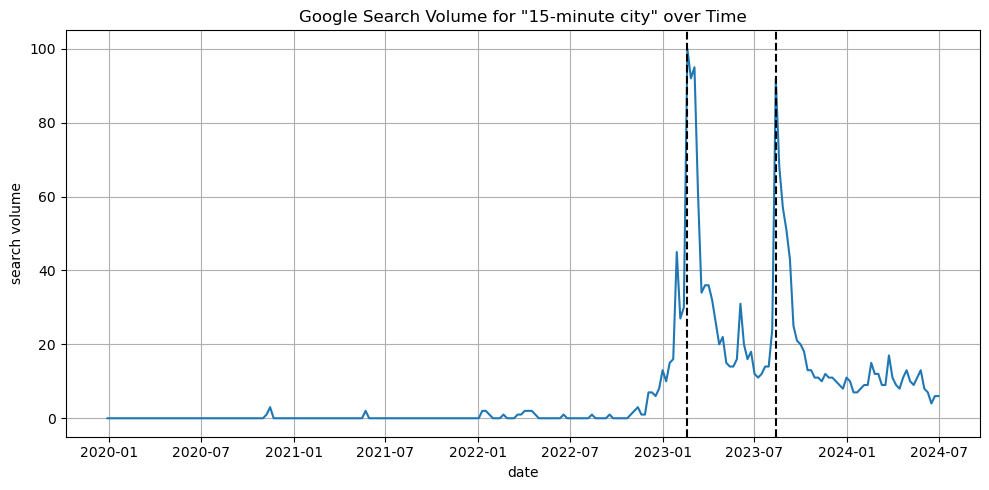
\includegraphics[width=0.8\textwidth]{img/gtrends_2-peak.png}
        \vspace{-5pt}
        \caption{Public interest in 15-minute cities measured by search volume}
        \vspace{-10pt}
        \label{fig:gtrends_raw}
    \end{figure}

    The results of the Google Trends data collection, visualized in Figure \ref{fig:gtrends_raw}, were crucial to the parametrization of the youtube api requests. Specifically, distinct phases centered around the presence or absence of a peak in public interest were algorithmically identified to ensure all relevant data was obtained while preventing excessive use of the api. For now, it is important to note that this procedure, the details of which will be discussed in \nameref{section:processing}, also yielded a cutoff-point before the first relevant phase.

    Following the google trends data collection, multiple endpoints of the YouTube Data Api were utilized to obtain relevant data on the most-viewed videos regarding 15-minute cities. First, the \textit{search} endpoint was employed to identify the 50 most-viewed videos per week. This weekly structure, while quota-intensive, enabled the identification of temporal trends in the analysis stage and was thus crucial for this project. Afterwards, metadata on all of the identified videos was obtained using the \textit{video} endpoint. Finally, multiple queries to the \textit{commentThread} endpoint per video allowed for the collection of all top-level comments under all videos. In total, 119 weeks of videos were processed, resulting in a dataset containing information on 2943 videos and 204093 comments, a process that required multiple days due to the quota limits imposed by the YouTube Data API.

    Finally, the huggingface api was utilized to obtain the LEIA-base transformer model \parencite{aroyehunLEIALinguisticEmbeddings2023}, which was later employed to classify the sentiments of the comments obtained via the YouTube Api. In addition to its performance in the assignments completed for this course, the LEIA-base model was chosen due to its ability to classify natural language sentiment in a fine-grained manner, distinguishing between Affection, Happiness, Anger, Sadness and Fear instead of a simple polarity score. This distinction of LEIA when compared to other sentiment analysis techniques such as VADER \parencite{cjhuttoVaderSentiment2020} is especially relevant in the context of conspiracy theories, as a comment expressing sadness implies a much lower threat level than a comment expressing anger. Thus, utilizing LEIA-base enables the generation of additional inferences into the conspiracy by providing a more fine-grained perspective.

\section{Data Processing}
\label{section:processing}

    \textcolor{red}{Explain how you filtered data, normalized values, computed additional variables, etc.}

    The Google Trends data  was utilized to identify distinct phases in public interest, with the goal of identifying connections to the development of the conspiracy theory. 

    \begin{figure}{}
        \centering
        \setlength\intextsep{0pt}
        \vspace{-30pt}
        \caption{} % leave empty, will print "Figure x" above it
        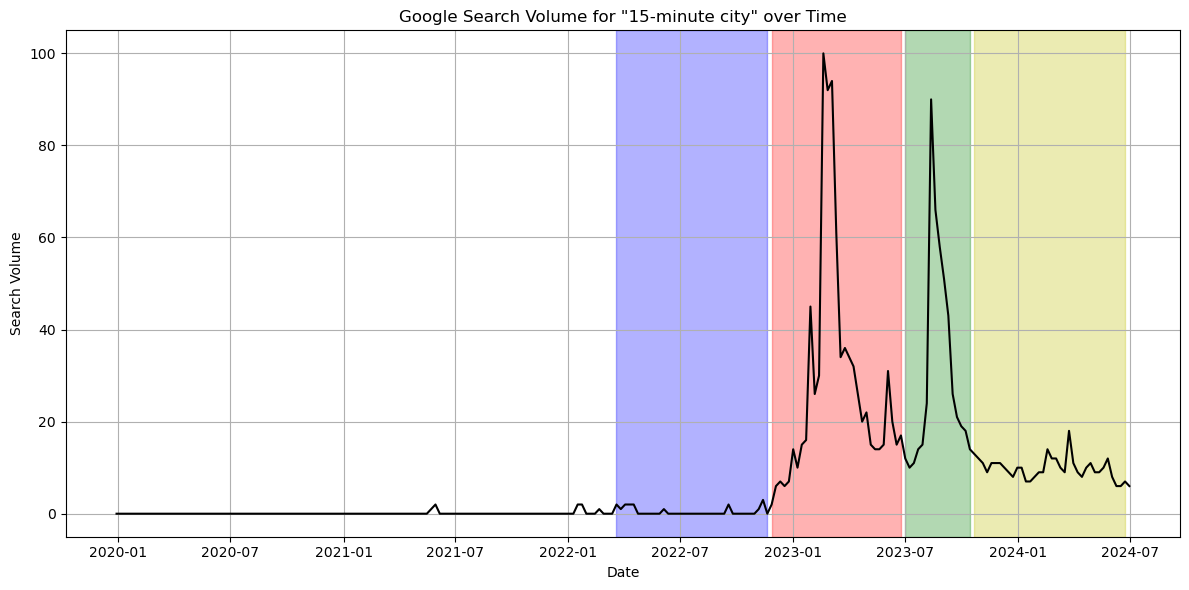
\includegraphics[width=0.8 \textwidth]{img/gtrends_phases.png}
        \vspace{-5pt}
        \caption*{Visualization of the generated phases}
        \vspace{-20pt}
        \label{fig:gtrends_phases}
    \end{figure}
    
\section{Analysis}
\label{section:analysis}

    \textcolor{red}{Perform statistical analyses and visualizations that assess the question(s).}

\section{Conclusion}
\label{section:conclusion}

    \textcolor{red}{Evaluate answers to the question and their reliability.}

\section{Critique}
\label{section:critique}

    \textcolor{red}{Identify limitations and alternative explanations for your results.}

    Further research points: 
-what was the “spark” leading conspiracy-prone accounts to this topic? (e.g., inclusion of measure in 2020 campaign by Paris mayor Anne Hidalgo – but conspiracies mainly emerging 3 years later?)
-Hypothesis: theories were driven by accounts already engaged in the “conspiracy bubble”

\newpage

\onecolumn
\begin{minipage}[t]{\textwidth}
    \printbibliography[heading=bibintoc, title={References}]
\end{minipage}


\end{document}
